\setAuthor{Stanislav Zavjalov}
\setRound{lahtine}
\setYear{2010}
\setNumber{G 7}
\setDifficulty{7}
\setTopic{Elektrostaatika}

\prob{Kärbes}
Kärbes on otsustanud
lennates püsida ainult ekvipotentsiaalsete pindade peal. Ta lendab sisse ruumi,
mis on täidetud homogeense elektriväljaga $\vec{E}$, välja jõujoontega risti.
Elektriväljas hoitakse paigal ka laengut $-Q$ nii, et kärbse
trajektoori esialgse puutuja ja laengu vahemaa on $d$ (vt. joonist; $-Q < 0$).
Kui lähedale kärbes laengule jõuab? Eeldage, et $Q \le \pi\epsilon_0Ed^2$.
\begin{center}
	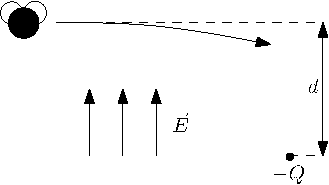
\includegraphics[width=0.4\textwidth]{2010-lahg-07-muha_tekst}
\end{center}

\hint
Kärbse potentsiaali on mugav avaldada $x-y$ koordinaadistikus. Ülesande sümmeetriast on suhteliselt lihtne näha, et kärbse kaugus laengust on minimaalne siis, kui ta asub otse laengu kohal.

\solu
Valime potentsiaali nullnivooks kärbse asümptootilise asukoha (lõpmatuses). 
Olgu laeng $Q$ koordinaatide alguspunktiks ning olgu $x$-telg horisontaalne ja $y$-telg vertikaalne. 
Kärbes peab püsima laengu lähedal kõverduval null-potentsiaalil. 
Potentsiaal avaldub homogeense välja $E$ potentsiaali ja punktlaengu potentsiaali superpositsioonina, seega 
\[
E(d - y) - \frac{1}{4\pi\epsilon_0}\frac{Q}{\sqrt{y^2 + x^2}} = 0.
\]
Ülesande sümmeetriast on selge, kärbse vahemaa on minimaalne $x=0$ korral, ehk teisisõnu kehtib $E(d-y) = kQ/y$. Antud võrrandist saame ruutvõrrandi lahenditega
\[
y_{1,2} = {d \over 2} \pm \sqrt{\frac {d^2}4 - {kQ \over E}} = {d \over 2}\left( 1 \pm \sqrt{1 - 4kQ / Ed^2}\right).
\] 
Juhul kui laeng on väike, liigub kärbes ilmselgelt sirgjooneliselt. Ometigi leidub kaks lahendit. Lahendi kahesus tuleneb sellest, et laengu läheduses leidub samuti
null-potentsiaaliga suletud kõver. Laengu kasvades need kaks null-potentsiaaliga joont lähenevad üksteisele, kuni $Q=\pi\epsilon_0Ed^2$ juures 
puutuvad kokku ja edaspidi moodustub null-potentsiaalist juba üksainus kõver, mis kulgeb ümber laengu. 
Seega vastab kärbse trajektoor ruutvõrrandi suuremale lahendile:
$$y= {d \over 2}\left(1 + \sqrt{1 - {4kQ \over Ed^2}}\right).$$
\probend